\documentclass[12pt]{article}
\usepackage{mathtools,amssymb, amsthm, tikz}
\usetikzlibrary{intersections}
\usetikzlibrary{patterns}
\usepackage[margin=1in]{geometry}
\usepackage{url}
\usepackage{natbib}
\usepackage[colorlinks=true, linkcolor=black, urlcolor=blue, citecolor=blue]{hyperref}
\usepackage[T1]{fontenc}
\usepackage[utf8]{inputenc}
\usepackage{lmodern}
\usepackage{fontspec}
\setmainfont{Times New Roman}

\title{Sutherland-Hodgman algoritmus}
\author{Pintér Bálint}
\renewcommand{\contentsname}{Tartalomjegyzék}
\renewcommand{\bibsection}{\section*{Források}}
\newcommand{\teglalap}{
    \begin{tikzpicture}[scale=0.15, baseline=(current bounding box.center)]
        \draw[black] (0,0) -- (1.5,0) -- (1.5,1) -- (0,1) -- cycle;
    \end{tikzpicture}
}
\newcommand{\sokszog}{
    
\begin{tikzpicture}[scale=0.15, baseline=(current bounding box.center)]
        \draw[black] (0,0) -- (0.5,0) -- (1.2,0.8) -- (0,1) -- cycle;
    \end{tikzpicture}
}
\newcommand{\haromszog}{
    \begin{tikzpicture}[scale=0.15, baseline=(current bounding box.center)]
        \draw[black] (0,0) -- (1,0) -- (0.5,1) -- cycle;
    \end{tikzpicture}
}


\begin{document}
\maketitle
\newpage
\tableofcontents
\newpage

\section{Bevezetés}
A Sutherland-Hodgman algoritmus egy clipping algoritmus. Feladata, hogy levágja
az alakzatok látómezőn kívűl eső részeit. A teljesen kívül eső alakzatokat
elveti, a vágósíkokat metsző alakzatokat úgy vágja meg, hogy csak a látható
rész maradjon.
\begin{center}
    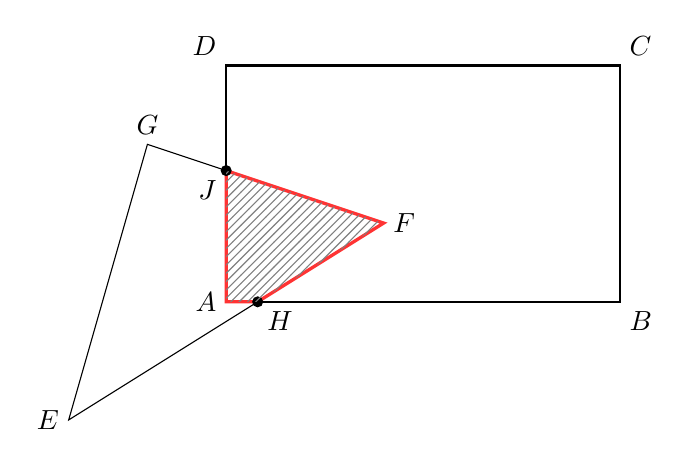
\begin{tikzpicture}
        \coordinate (A) at (0,0);
        \coordinate (B) at (5,0);
        \coordinate (C) at (5,3);
        \coordinate (D) at (0,3);
        \coordinate (E) at (-2,-1.5);
        \coordinate (F) at (2,1);
        \coordinate (G) at (-1,2);

        \draw[name path=rectangle, thick] (A) -- (B) -- (C) -- (D) -- cycle;
        \draw[name path=triangle] (E) -- (F) -- (G) -- cycle;
        \path [name intersections={of=rectangle and triangle, by={H, J}, sort by=rectangle}];
        \draw[very thick, red!80]
        (A) -- (H) -- (F) -- (J) -- cycle;

        \fill [black] (H) circle (2pt) node[below right] {$H$};
        \fill [black] (J) circle (2pt) node[below left] {$J$};

        \fill[pattern=north east lines, pattern color=gray]
        (A) -- (H) -- (F) -- (J) -- cycle;

        \node[left] at (A) {$A$};
        \node[below right] at (B) {$B$};
        \node[above right] at (C) {$C$};
        \node[above left] at (D) {$D$};

        \node[left] at (E) {$E$};
        \node[right] at (F) {$F$};
        \node[above] at (G) {$G$};

    \end{tikzpicture}
    \\
    \textbf{1. Ábra:}\\Sutherland-Hodgman algoritmus szemléltetése \\ $ABCD_{\teglalap}$ vágósokszög\\$EFG_{\haromszog}$ Levágandó sokszög\\$AHFJ{\sokszog}$ Levágott sokszög
\end{center}
\section{Az algoritmus}
\subsection{Vágótér (clip space)}
A levágást perspektív mátrixszal való szorzás után, de a perspective divide
előtt végezzük homogén koordinátákkal. Ez a clip space. A perspektív mátrixszal
való szorzás előtt a látótér egy csonkagúla (viewing frustum). A perspektív
mátrixszal való szorzás után egy kocka, amin a vágási feltételek egyszerűen
vizsgálhatók. Clip spaceben végezzük a levágást, mert camera spaceban a látótér
egy csonkagúla, amire nehéz lenne vágni. A perspective divide után a kamera
mögötti pontok (melyekre $w\leq0$) helytelenül vetítődnek a képernyőre, ezért a
vágást a perspective divide előtt kell elvégezni.
\subsection{A vágás lépései}
Egy sokszöget a pontjai megadott sorrendje határozza meg. A sokszög oldalait
teszteljük a síkhoz képest. Az oldalnak négy lehetséges elhelyezkedése van a
síkhoz képest:
\begin{enumerate}
    \item \textbf{(BE$\rightarrow$BE)} Mindkét pontja belül van
    \item \textbf{(BE$\rightarrow$KI)} Kezdeti pontja belül van, de a végpontja kívül van
    \item \textbf{(KI$\rightarrow$BE)} Kezdeti pontja kívül van, de a végpontja belül van
    \item \textbf{(KI$\rightarrow$KI)} Mindkét pontja kívül van
\end{enumerate}
A pontokról clip spaceben egyszerű elsőfokú egyenlőtlenséggel el lehet dönteni, hogy a sík
melyik oldalán van (mivel egy kocka). A perspektív mátrixunk úgy lett megírva,
hogy $x,y\in[-1;1]$ és $z\in[0;1]$. A perspective divide előtt ($w$-vel osztás) a koordinátáink:
\begin{align*}
    -w & \leq x \leq w \\
    -w & \leq y \leq w \\
    0  & \leq z \leq w \\
\end{align*}
Így a feltételeink a kocka különböző oldalaira:
\begin{center}
    \begin{tabular}{|c | c | c |}
        \hline
        \parbox{0.25\linewidth}{
            \vspace{4pt}
            \textbf{Jobb oldali sík:}
            \[
                \begin{aligned}
                    x & \leq w     \\
                    0 & \leq w - x
                \end{aligned}
            \]
        } &
        \parbox{0.25\linewidth}{
            \vspace{4pt}
            \textbf{Felső oldal síkja:}
            \[
                \begin{aligned}
                    y & \leq w     \\
                    0 & \leq w - y
                \end{aligned}
            \]
        } &
        \parbox{0.25\linewidth}{
            \vspace{4pt}
            \textbf{Távoli oldal síkja:}
            \[
                \begin{aligned}
                    z & \leq w     \\
                    0 & \leq w - z
                \end{aligned}
            \]
        }   \\
        \hline
        \parbox{0.25\linewidth}{
            \vspace{4pt}
            \textbf{Bal oldali sík:}
            \[
                \begin{aligned}
                    -w & \leq x     \\
                    0  & \leq x + w
                \end{aligned}
            \]
        } &
        \parbox{0.25\linewidth}{
            \vspace{4pt}
            \textbf{Alsó oldal síkja:}
            \[
                \begin{aligned}
                    -w & \leq y     \\
                    0  & \leq y + w
                \end{aligned}
            \]
        } &
        \parbox{0.25\linewidth}{
            \vspace{4pt}
            \textbf{Közeli oldal síkja:}
            \[
                \begin{aligned}
                    0 & \leq z
                \end{aligned}
            \]
        }   \\
        \hline
    \end{tabular}
\end{center}
\newpage
\nocite{*}
\bibliographystyle{plainnat}
\bibliography{forrasok}

\end{document}